\documentclass{article}

\usepackage{xltxtra} % Loads fontspec, xunicode, metalogo, fxltx2e, and some extra customizations for XeLaTeX
%\defaultfontfeatures{Mapping=tex-text} % to support TeX conventions like ``---''
\defaultfontfeatures{Mapping=tex-text}
\setmainfont{Cambria}
\usepackage{csquotes}
\usepackage{graphicx}
\usepackage[margin=2.5cm]{geometry}
\newcounter{boardcounter}
\setcounter{boardcounter}{0}
%This command numbers frames and adds two blank lines for annotation.
\newcommand{\Annotate}{\stepcounter{boardcounter}[\arabic{boardcounter}]\vspace{\baselineskip}
\rule{\linewidth}{1pt}\\
\rule{\linewidth}{1pt}
\vspace{2\baselineskip}
\vfill
}
%Toggle to display subtitles in a different language
%\newcommand{\Bislama}[1]{#1}
\newcommand{\Bislama}[1]{}
%\newcommand{\English}[1]{}
\newcommand{\English}[1]{#1}
\newcommand{\Daakaka}[1]{}
%\newcommand{\Daakaka}[1]{#1}

\begin{document}
\center 
{\huge \Bislama{Lafet wantaem}\English{Festival}} 
\vfill

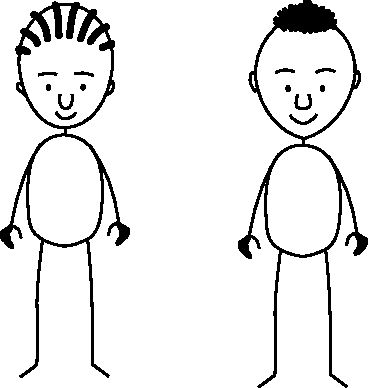
\includegraphics[scale=.7]{StoryboardsFestival01}

\Bislama{Hemia Sam, hemia Luk. Tufala i fren.}
\English{This is Sam, this is Luke. The two are friends}
\Daakaka{Temeli man nya lo, saya is sa Josef ten Jason.}

\Annotate

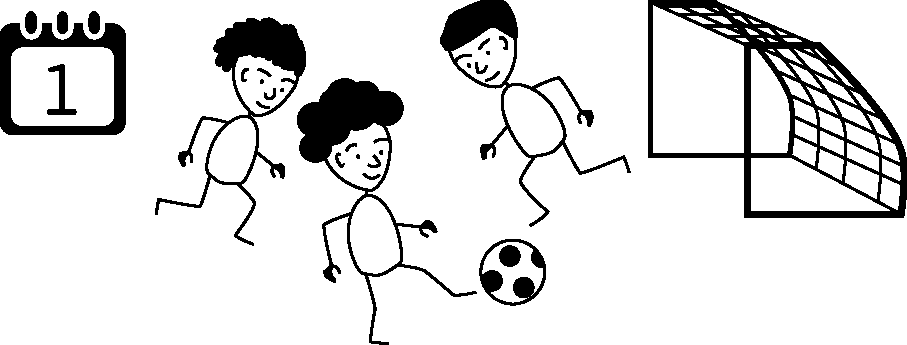
\includegraphics[width=.4\linewidth]{StoryboardsFestival02.pdf}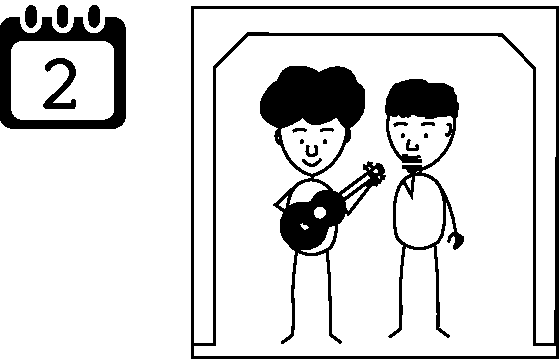
\includegraphics[width=.25\linewidth]{StoryboardsFestival03} 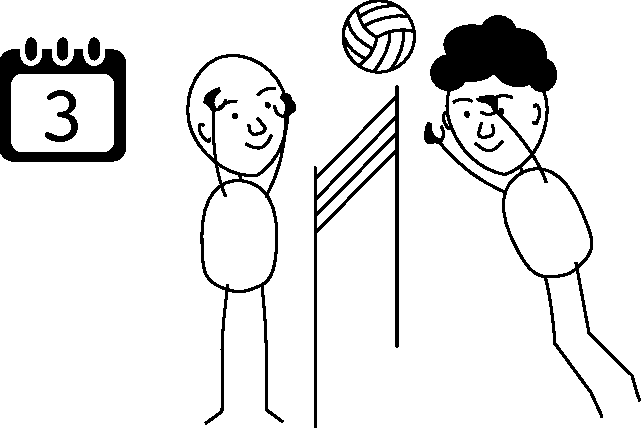
\includegraphics[width=.25\linewidth]{StoryboardsFestival04.pdf}

\Bislama{Long ples blong tufala i gat tri de blong lafet wetem ol pleple.}
\English{There is a three-day festival in Ŋukurr --- the place where they live.}
\Daakaka{Bangbangan pwer webung sii kuane nya.}

\Annotate

\pagebreak
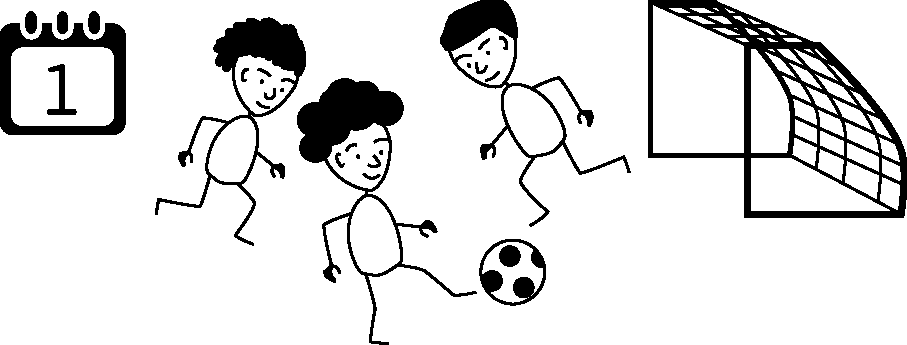
\includegraphics[scale=.7]{StoryboardsFestival02}

\Bislama{Long fes de i gat wan gem blong futbol.}
\English{On the first day, there is a game of soccer.}
\Daakaka{Webung na mwi mo yam ple futbol.}

\Annotate

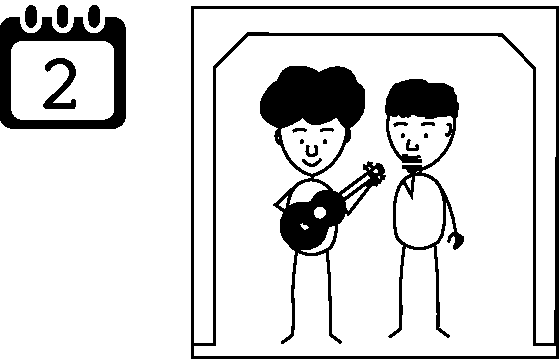
\includegraphics[scale=.7]{StoryboardsFestival03}

\Bislama{Long seken de i gat wan konset.}
\English{On the second day, there is a concert.}
\Daakaka{Webung lo an yam gene konset.}

\Annotate

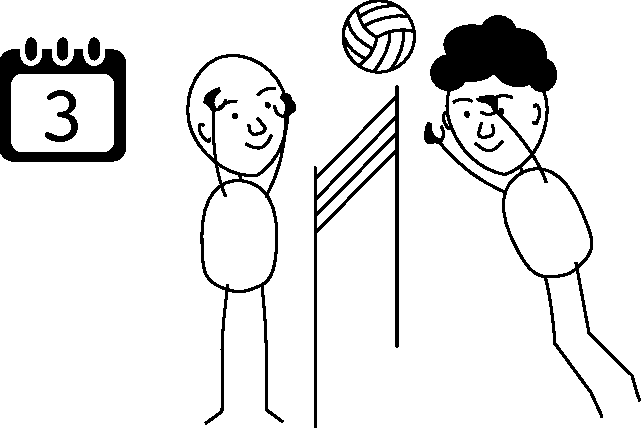
\includegraphics[scale=.7]{StoryboardsFestival04}

\Bislama{Long ted de i gat wan gem blong volibol.}
\English{On the third day, there is a volleyball game.}
\Daakaka{Webung sii an yam bangbangane volibol.}

\Annotate

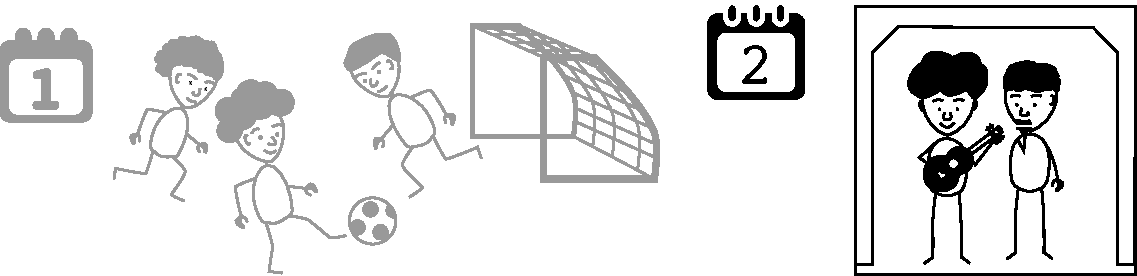
\includegraphics[width=\textwidth]{StoryboardsFestival05.pdf}

\Bislama{De blong futbol i go finis. Tede hem i seken de blong lafet, we i gat konset.}
\English{The day of the soccer game has already passed. Today is the second day of the festival, on which there is a concert.}
\Daakaka{Webung mo an mwe vyan mo nok, yam du ongane konset.}

\Annotate

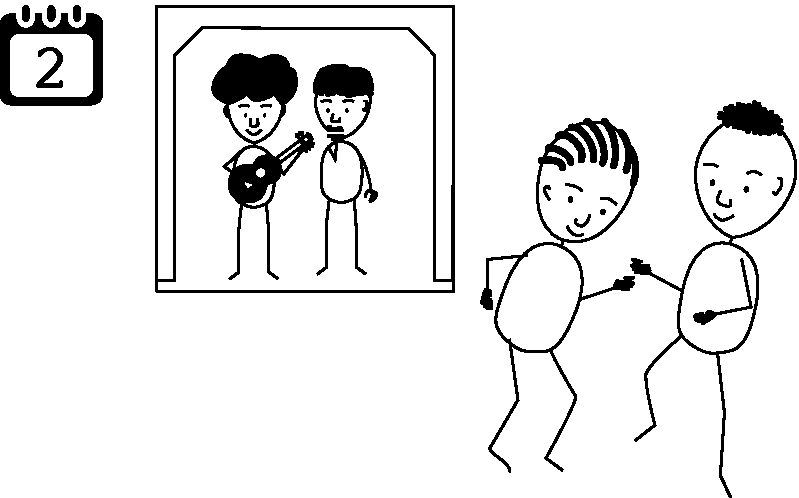
\includegraphics[scale=.7]{StoryboardsFestival06.pdf}

\Bislama{Luk mo Sam tufala i stap danis long konset ia. Tufala i stap tokbaot lafet.}
\English{Luke and Sam are dancing at the concert. The two are talking about the festival.}
\Daakaka{Yem du sap.}

\Annotate
\pagebreak

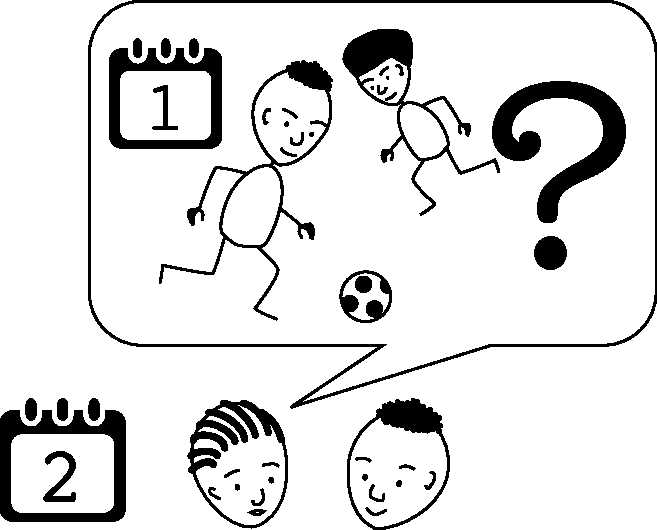
\includegraphics[scale=.7]{StoryboardsFestival07.pdf}

\Bislama{Nao ia, Sam i stap askem Luk, hem i se: \enquote{Yestede yu ple futbol?}}
\English{Now Sam asks Luke: \enquote{Did you play soccer yesterday?}}
\Daakaka{Josef ma usi ane Jason: Nenyu kom bangbangane futbol mwede?}

\Annotate
	
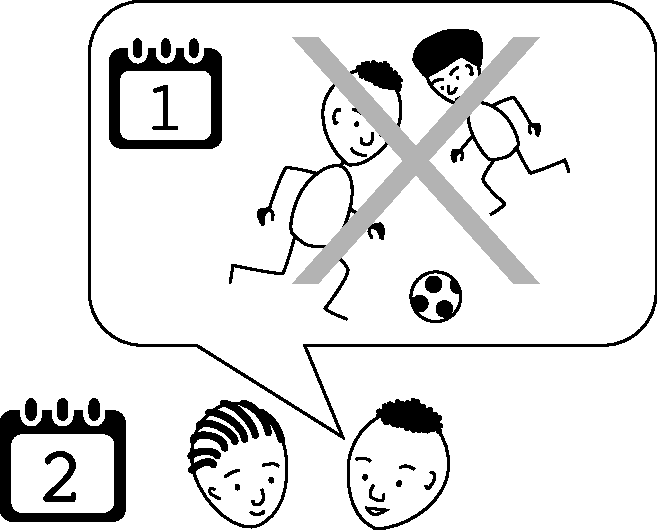
\includegraphics[scale=.7]{StoryboardsFestival08.pdf}

\Bislama{Ale Luk hemi se: \enquote{No, yestede mi no bin ple.}}
\English{The Luke says: \enquote{No, I didn't play yesterday.}}
\Daakaka{}

\Annotate
\pagebreak

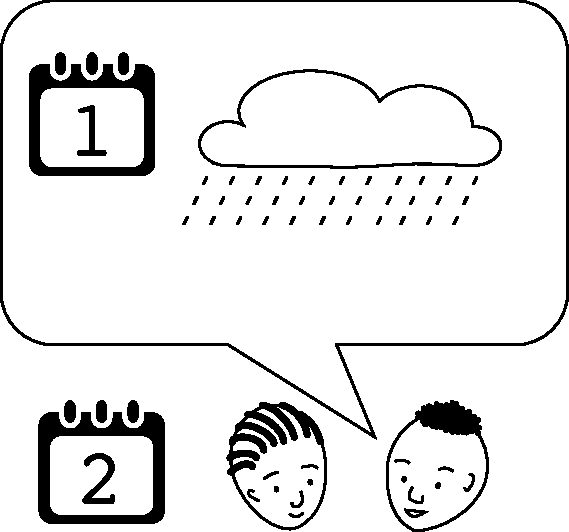
\includegraphics[scale=.7]{StoryboardsFestival09.pdf}

\Bislama{Hemi se: \enquote{Yestede, ren i ren.}}
\English{He explains: \enquote{Yesterday it was rainy.}}

\Annotate


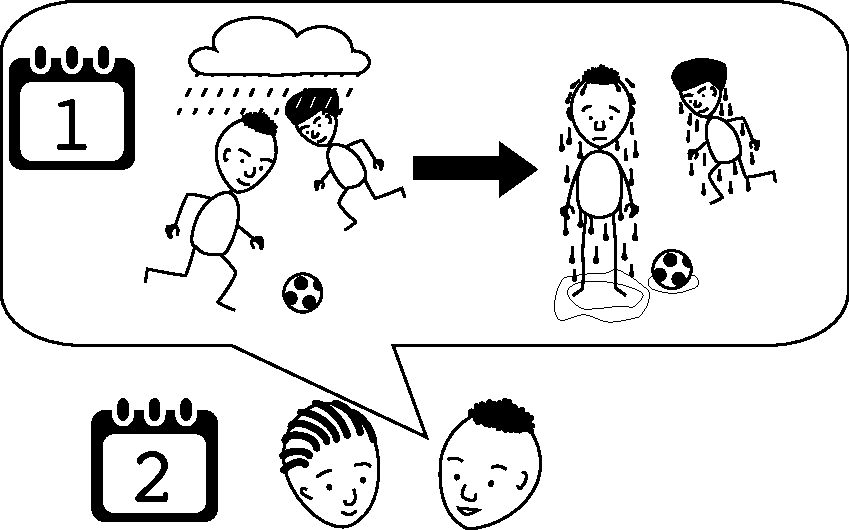
\includegraphics[scale=.7]{StoryboardsFestival10.pdf}

\Bislama{Hemi se: \enquote{Sapos mi bin ple futbol yestede, bae mi wetwet.}}
\English{He says: \enquote{If I had played soccer yesterday, I would have gotten wet.}}

\Annotate
\pagebreak

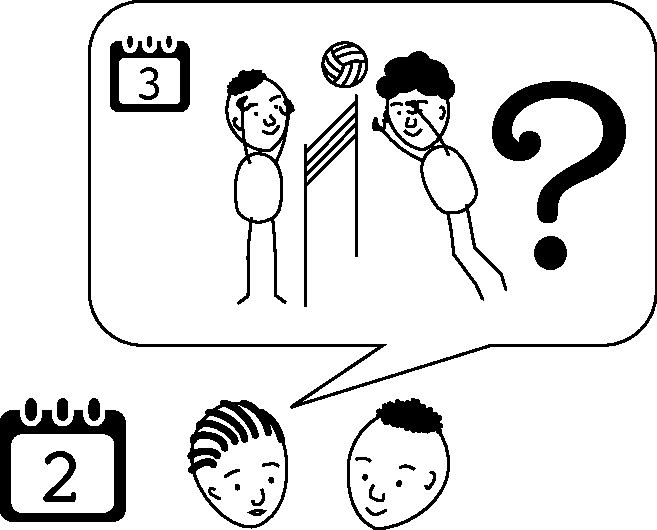
\includegraphics[scale=.7]{StoryboardsFestival11.pdf}

\Bislama{Afta Sam hemi askem se: "Ale, tumoro, bae yu ple volibol?"}
\English{Then Sam asks: "So will you play volleyball tomorrow?"}

\Annotate

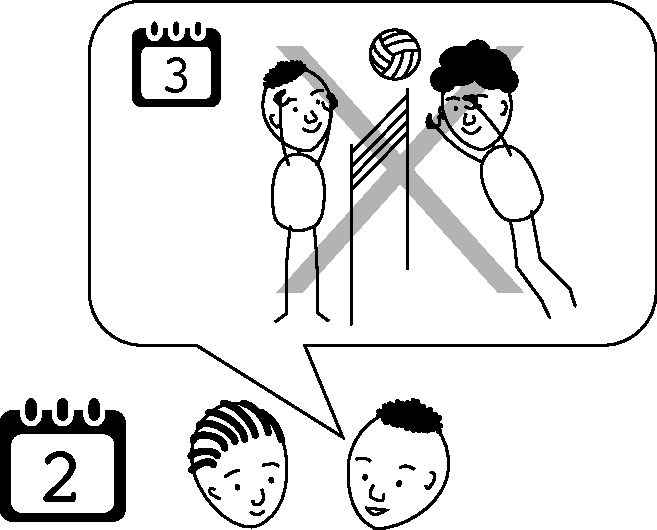
\includegraphics[scale=.7]{StoryboardsFestival12.pdf}

\Bislama{Ale Luk hemi se: "No, bae mi no ple."}
\English{Then Luk says: "No, I won't play."}

\Annotate
\pagebreak

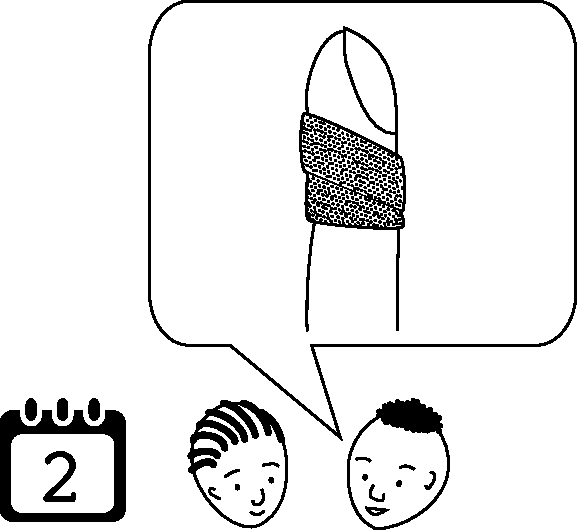
\includegraphics[scale=.7]{StoryboardsFestival13.pdf}

\Bislama{Hemi explenem: "Mi bin katem finga blong mi."}
\English{He explains: "I cut my finger."}

\Annotate


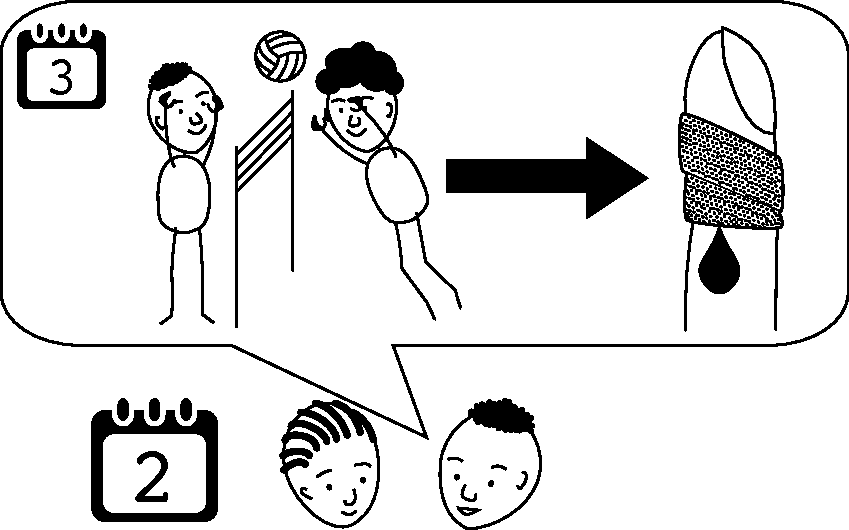
\includegraphics[scale=.7]{StoryboardsFestival14.pdf}

\Bislama{Luk hemi se: "Sapos bae mi ple volibol tumoro, bae soa blong finga blong mi bae brok bakegen."}
\English{He says: ``If I played volleyball tomorrow, the wound would come open again."}

\Annotate
\pagebreak

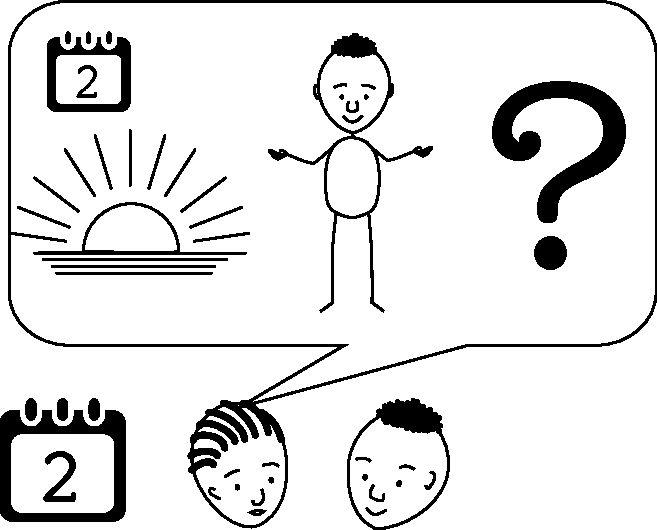
\includegraphics[scale=.7]{StoryboardsFestival15.pdf}

\Bislama{Afta Sam hemi askem Luk: "Tede long naet bambae yu mekem wanem?"}
\English{The Sam asks Luk: "What are you going to do tonight?"}

\Annotate

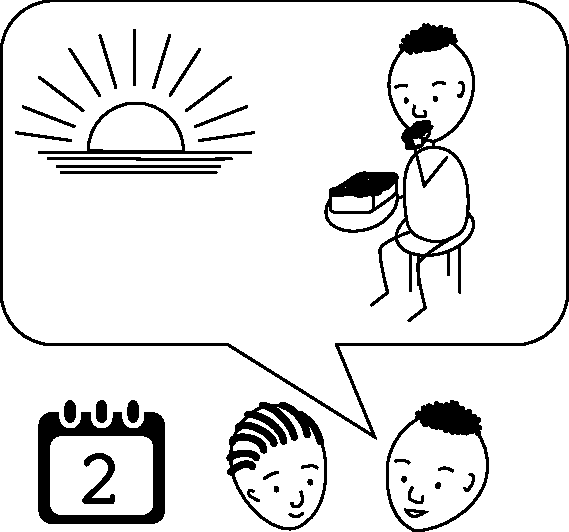
\includegraphics[scale=.7]{StoryboardsFestival16.pdf}

\Bislama{Luk hemi talem se: ``Long naet bae mi kakae plante laplap!"}
\English{Luk says: ``At nighttime, I will eat lots of cake!"} %Outside of a Melanesian setting you can change this to cake/lasagna/quiche etc.

\Annotate 
\pagebreak

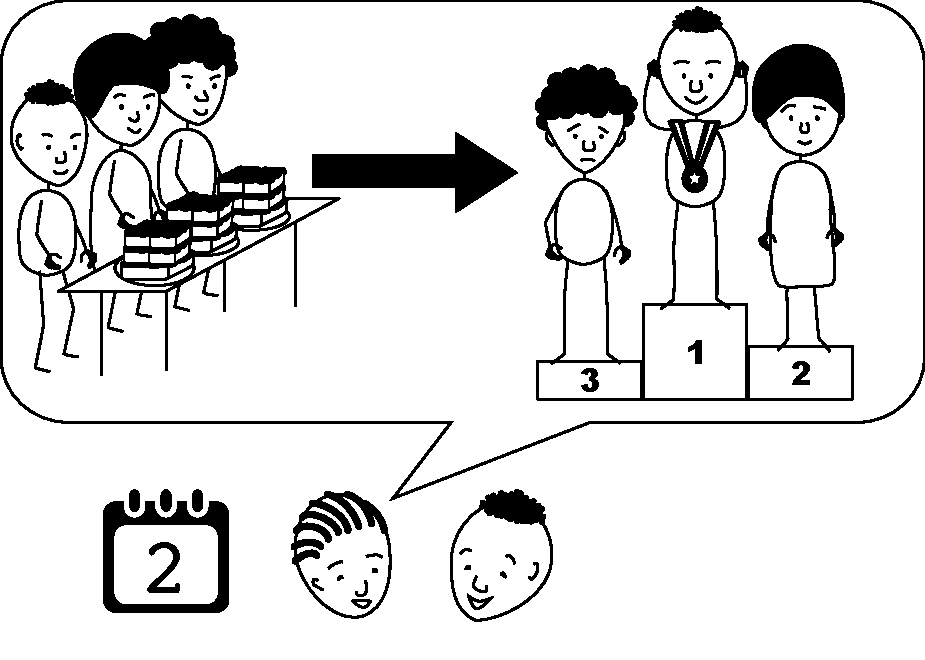
\includegraphics[scale=.7]{StoryboardsFestival17.pdf}

\Bislama{Ale Sam hemi se: "Sapos i gat kompetesen blong kakae laplap, bae yu winim wantaem!"}
\English{Then Sam says: "If there was a cake-eating competition, you would definitely win it!"}

\Annotate 

\end{document}